\section{Systembeskrivning}

% Systemet funktion vid starten är att öka oftare i början bootstrapen
% (exempelvis innan målgivaren) för att sedan öka mindre frekvent i segment 1.
% Bootsrapen (uppstarten) avslutas efter segment 3. 

\begin{figure}
	\centering
	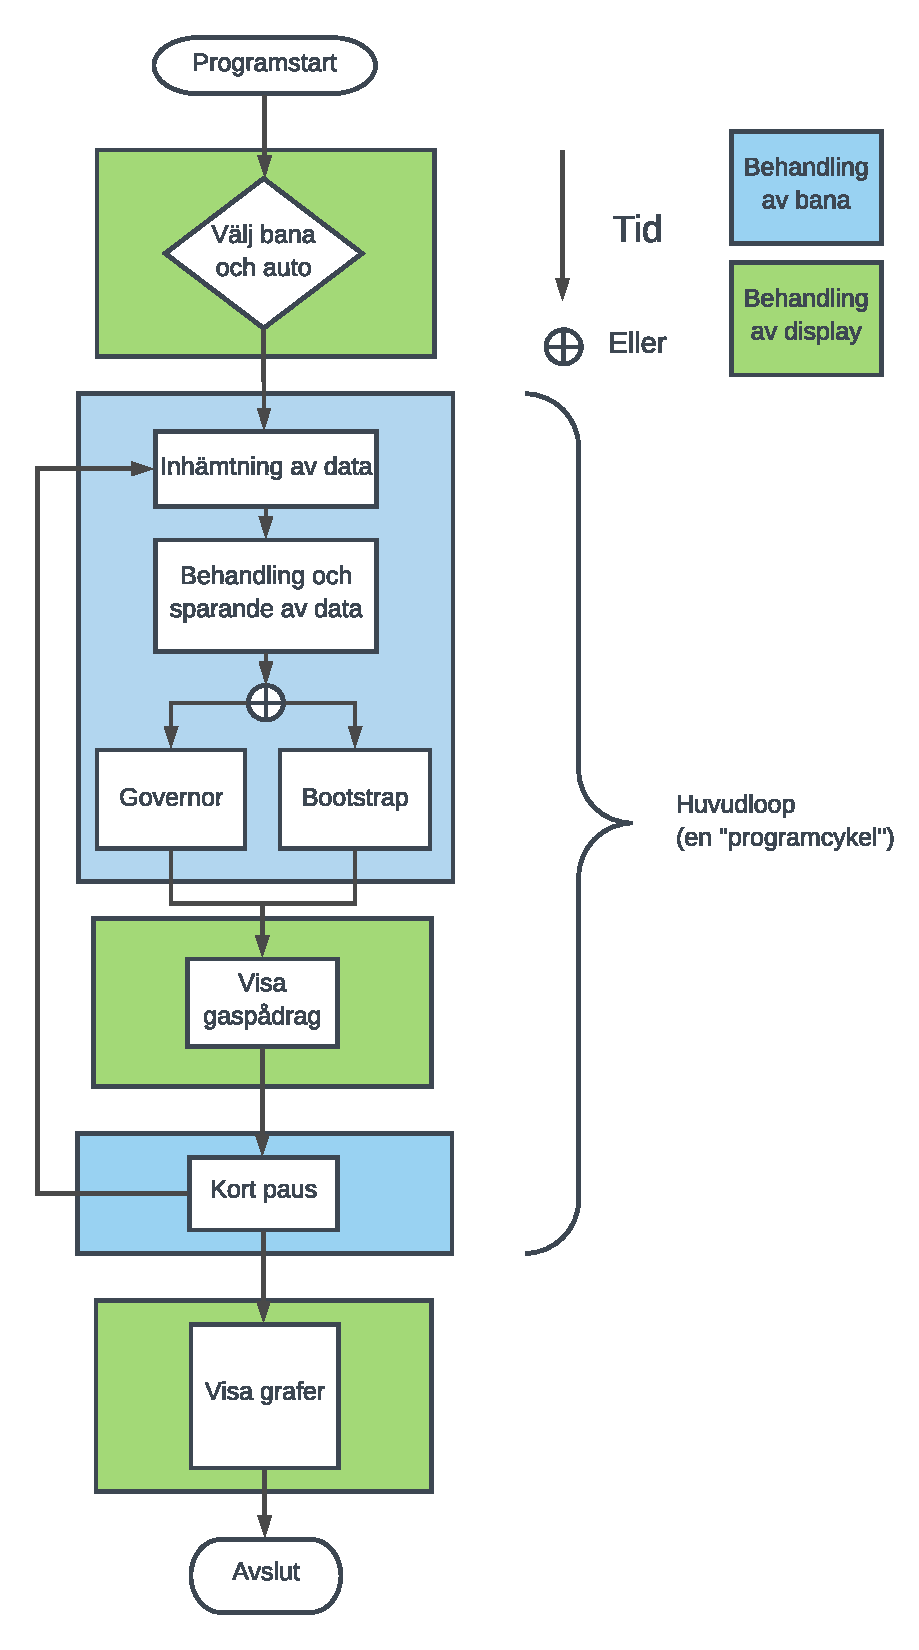
\includegraphics [height=0.8\textheight] {Figures/flow}
	\caption{Flödesschema över systemet.}
	\label{fig:flow}
\end{figure}

Systemet är indelat i 2 delsystem, bana och display. Delsystemen är indelade i olika delmoment efter huvudsaklig funktionalitet enligt Figur
\ref{fig:flow}. Nedan beskrivs dessa delmoment i mer detalj.

\subsection{Innan start}

Vid uppstart ritas knappar ut på displayen, se figur x. Med dessa knappar går
det att välja om en eller två banor ska vara aktiva och om de ska styras
autonomt av systemet eller manuellt med handkontroll. Det går också att ställa
in en referenstid mellan 12 och 15 sekunder med 0,5 sekunders intervall genom
att trycka på + och - på displayen. 

\subsection{Uppstart} 
\label{sec:systembeskrivning:uppstart}
Vid autonom körning utgår systemet ifrån en bootstrap som är till för uppstarten av bilarna. Då körs funktionen \texttt{do\_boot()} som arbetar fram en
initial \texttt{car.constant}. Detta sker i tre steg. Innan bilen börjar rulla
höjs \texttt{car.constant} varje 0,7 sekunder. När bilen börjar rulla och åker
under målgivaren höjs \texttt{car.constant} långsammare tills bilen åkt under
den första givaren varpå \texttt{car.constant} inte längre ändras. Vid den
tredje givaren jämförs hur lång tid det senaste segmentet tog att köra och en
sista \texttt{car.constant} räknas ut som förväntas ge en varvtid på 15
sekunder. Om den förväntade varvtiden är längre än 15 sekunder höjs
\texttt{car.constant} och om den förväntade varvtiden är lägre sänks
\texttt{car.constant}.

\subsection{Körning}
\label{sec:systembeskrivning:korning}

Körningen är uppdelad i olika faser. Dessa presenteras nedan. En
\emph{programcykel} är när dessa faser körs igenom en gång. Samlingsnamnet för
faserna är \emph{huvudloopen}. Systemet behöver köra programcykler med som högst
0,1~sekunders intervall (enligt krav 31). I en programcykel beräknar systemet
var bilen befinner sig, hur snabbt bilen ska köra och skickar det nya
gaspådraget till banan. När en givare passeras justeras också bilens konstant
efter nuvarande varv- och referenstid.  Nedan beskrivs vad systemet gör under en
komplett programcykel.

\subsubsection{Position}
\label{sec:system:korning:position}

Om en givare passerats vet systemet exakt var bilen befinner sig. Om så är
fallet sparas den nuvarande exakta position och kallas \emph{givarpositionen}.

% Om en ny givare har passerats, \texttt{car.new\_check\_point == true}, ökar
% programmet nuvarande segment (\texttt{car.segment}) med 1. \texttt{car.segment}, som
% alltid ligger mellan 1 och 9, används som index för att välja position i en
% lista (\texttt{car.pos\_at}). Vi kallar den positionen för \emph{givarpositionen}.

Oavsett om en givare passerats eller inte räknar systemet ut en beräknad
position. Detta görs genom att räkna ut en approximativ hastighet $v =
\frac{s}{t}$ där $v$ är hastigheten, $s$ är längden på det nuvarande segmentet
och $t$ är hur lång tid det nuvarande segmentet tog förra varvet.

% Om ingen givare har passerars och första varvet är avslutat kallas först på
% funktionen \texttt{get\_approx\_v()}. Denna utgår ifrån förra varvets
% segmentstider (\texttt{car.seg\_times}) och segmentslängder
% (\texttt{car.seg\_len}) och beräknar med $v = \frac{s}{t}$, där \texttt{s} är
% segmentslängden och \texttt{t} segmentstiden, \texttt{v} som är
% medelhastigheten för nuvarnade segment, men förra varvet. Denna antas vara
% ungefär samma som nuvarande hastiget och kallas \emph{car.v}. 

Med den approximativa hastigheten räknar sedan systemet ut hur långt bilen rört
sig sen den senaste programcykeln. Denna förflyttning räknas ut med $\mathrm{d}s
= v \cdot \mathrm{d}t$ där $\mathrm{d}s$ är den beräknade förflyttningen, $v$
hastigheten som precis räknades ut och $\mathrm{d}t$ tiden sedan den förra
programcykeln. Denna förflyttning läggs till positionen från förra programcykeln
och kallas den \emph{beräknade} positionen.

Om en givare passerats upskattar systemet sedan om en givare vid ett tidigare
tillfälle passerats (genom att jämföra givarpositionen och den beräknade
positionen). Information om denna procedur finns i del~\ref{sec:missade givare}.

% Sedan beräknas positionen, i meter från målgivaren, med funktionen
% \texttt{get\_position()}. Den använder den ungefärliga hastigheten \texttt{v} beräknad av
% \texttt{approx\_v()} och tiden \texttt{t} sedan denna beräkning gjordes senast (en programcykel, se \ref{sec:system:korning:cykel})
% och beräknar med $s = v \cdot t$ den sträcka som bilen har åkt. Sedan adderas denna
% med förra kända positionen och returneras i \texttt{car.position}. Denna 
% \emph{beräknade} position tas också fram när en givare har passerats, då skrivs den över med \emph{givarpositionen} men används i stället för att detektera missade givare. Se \ref{sec:missade givare}.

\subsubsection{Gaspådrag}

Efter positionsberäkningen beräknas spänningen som ska skickas till banan. Först används positionen för att välja en spänningsparameter. Denna finns i kartan som är indexerad efter position. Gaspådraget ($u$) fås sedan genom att multiplicera denna hastighetsparameter ($v$) med bilens konstant ($k$): $u = v \cdot k$.

% Efter positionsberäkningen beräknas det gaspådrag som skall sättas till banan. Detta görs i två
% funktioner, \texttt{get\_new\_v} och \texttt{get\_new\_u}.
% 
% I \texttt{get\_new\_v} används bilens nuvarande postition (\texttt{car.postition})
% och hastighetskartan (\texttt{car.map}). I \texttt{car.map} finns en
% hastighetsparameter för varje \texttt{car.position} (Se \ref{sec:begrepp och systemöversikt}.), denna retuneras av funktionen
% och sparas i \texttt{car.v}.
%  
% I \texttt{get\_new\_u} används denna hastighetsparameter tillsammans med
% \texttt{car.constant}. Dessa multipliceras och deras produkt retuneras och sparas
% i \texttt{car.u}.

\subsubsection{Governor}
\label{sec:systembeskrivning:governor}

Om bootstrap är avslutad och en givare passerats behöver bilens konstant
eventuellt justeras. För att justera bilens konstant behöver systemet först beräkna hur lång tid det
nuvarande varvet kommer ta. Vid varje givare beräknas därför den genomsnittliga
hastigheten genom det förra segmentet och multipliceras med den kvarvarande
sträckan på varvet för att få den uppskattade tiden den resterande delen av
varvet kommer ta. Denna tid läggs ihop med varvtiden hittils och ger då en
uppskattad varvtid för det nuvarande varvet. Denna varvtid jämförs sedan med den
valda referenstiden och bilens konstant anpassas vid behov.

% Detta görs med funktionen \texttt{do\_gov}.  Först görs en uppskattning av 
% varvtiden utifrån hur lång tid varvet har tagit än
% så länge. Detta görs med forecasts som beräknar den approximerade varvtiden utifrån tid fram tills senast
% passerad givare samt hastighet i tidigare segment. Genom att veta en
% genomsnittlig hastighet går det med kvarvarande sträcka att räkna ut en
% ungefärlig kvarvarande tid. När tiden från mål till senaste passerade givare adderas med
% den uträknade approximerade tiden kvar, så erhålls det en uppskattad varvtid som
% används för att avgöra om en bil behöver åka snabbare eller långsammare. Om bilen dock är inne på sitt första varv görs uppskattningen endast
% utifrån förra segmentet \texttt{car.forcasts\_naive} och om första varvet är
% avslutat så används \texttt{car.forcasts} som vanligt. Detta görs efter segment 4 och 8. Dessutom används den
% faktiska varvtiden när bilen passerar mål (från varv 2 och frammåt).
%  
% Sedan jämförs denna uppskattade varvtid med referenstiden (\texttt{car.ref\_time}) 
% och \texttt{car.constant} justeras.

% \begin{verbatim}
% car.constant = car.constant + (status - 1) * 0.08;
% \end{verbatim}

% Där \texttt{status} är den uppskattade varvtidens förhållande till \texttt{car.ref\_time}.
% D.v.s om de är exakt lika blir \texttt{status~ =~ 1}, om uppskattningen är högre blir
% den större än 1 och om den är lägre blir den mindre än 1. Således kommer \texttt{car.constant}
% höjas eller sänkas proportionellt mot hur långt ifrån \texttt{car.ref\_time} uppskattningen
% av varvtiden ligger. 

\subsubsection{Hantering av längden av en programcykel}
\label{sec:system:korning:cykel}

I slutet av varje cykel körs en loop som tillfälligt pausar programmet.
För att få avläsningen att ske minst en gång var tionde sekund pausas
programmet kontinuerligt 0,001 sekunder tills den totala paustiden överskrider 
0,07 sekunder då nästa cykel börjar. Då pausen på 0,001 sekunder är så pass
kort och marginalen till kravet är rätt stor så sker avläsningen mellan
0,07 och 0,1 sekunder. Längden på den största skillnaden mellan två avläsningar
sparas och visas vid programmets slut.


\subsubsection{Display}

I varje programcykel skickas nuvarande värdet på u till två stapeldiagram på
displayen för vardera bil. Se appendix N för mer information om displayens
stapeldiagram. Om ett nytt varv har inletts skrivs dessutom varvnumret och
varvtiden ut på displayen.


\subsection{Avslut}

Om det har gått mer än nio sekunder sedan en givare passerades pausas programmet
och användaren informeras på styrdatorn att en bil misstänkts ha fastnat eller
åkt av banan. 

För att avbryta programmet manuellt kan användaren när som helst trycka på q
eller s på datorns tangentbord. Trycker användaren på q avslutas programmet
direkt. Trycker användaren på s stoppas varje bil var för sig när den uppskattas
befinna sig 80~cm framför målgivaren. Programmet avslutas när båda bilarna
stoppats.

När körningen avslutas slutar systemet skicka spänning till banan.  Om en bil
kört fler än två varv sparas statistik från körningen i en \texttt{.mat}-fil med
nuvarande datum och tid som filnamn. Vid programslut visas också statistik om
varvtid och genomsnittlig segmenttid på displayen (Figur~\ref{fig:display-seg}
och Figur~\ref{fig:display-lap}).

